\documentclass[14pt,hyperref={CJKbookmarks=true}]{beamer}
\usepackage{time}
\usepackage[space,noindent]{ctex}
\usepackage{multimedia}
\usepackage{times}
\usetheme{Madrid}
\setbeamercolor{background canvas}{bg=}  %ˮӡ

\begin{document}
\songti
\zihao{5}
%\title{�������ֵشŴ�����}
\title{Three-Axis Digital Magnetometer}
\author{���}
\institute{Apollo-Rescue��Automation, NJUPT}
\date{2011.12.16}

\section{Introduction}
\begin{frame}
\titlepage
\end{frame}

\begin{frame}
    \begin{center}
       {\zihao{1} ?}
    \end{center}

\end{frame}

\begin{frame}
    \begin{columns}[onlytextwidth]
        \begin{column}{0.5\textwidth}
        
        ����شų�������\\
        %MAG3110��Xtrinsic�߾���3�������
        \end{column}
    \begin{column}{0.5\textwidth}
            %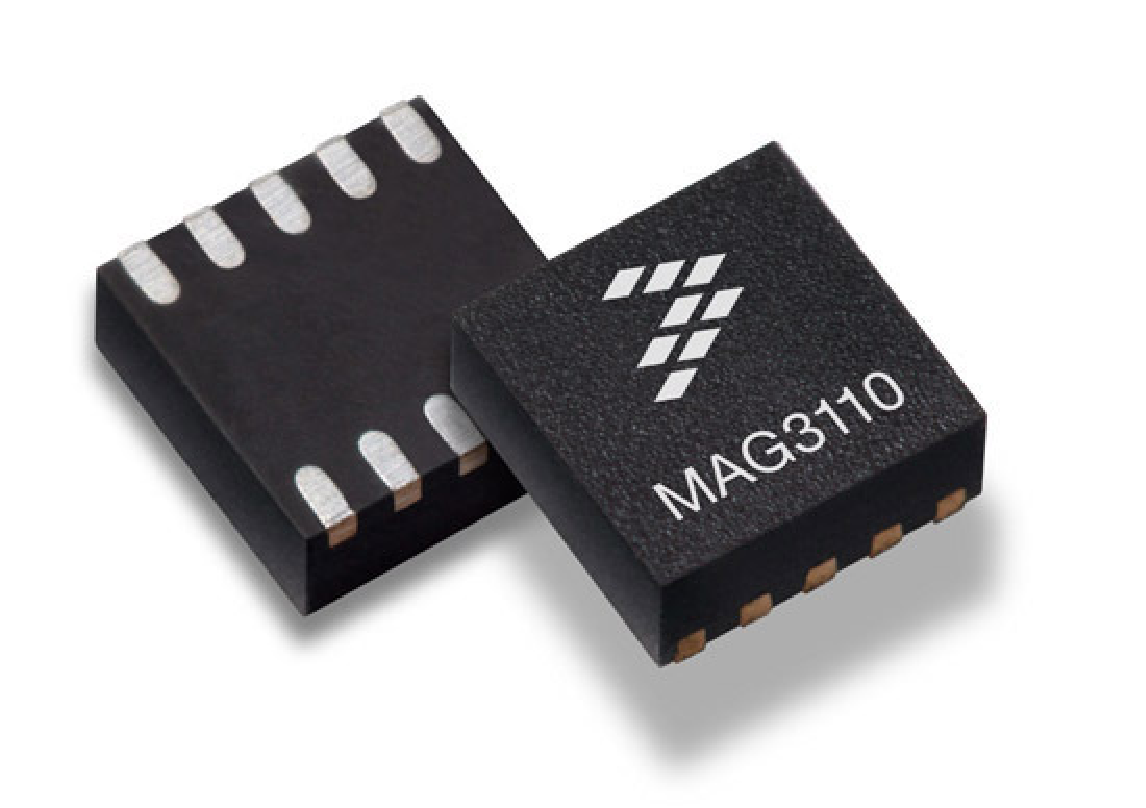
\includegraphics[height=45mm,width=\columnwidth]{MGA}\\
        \begin{center}
            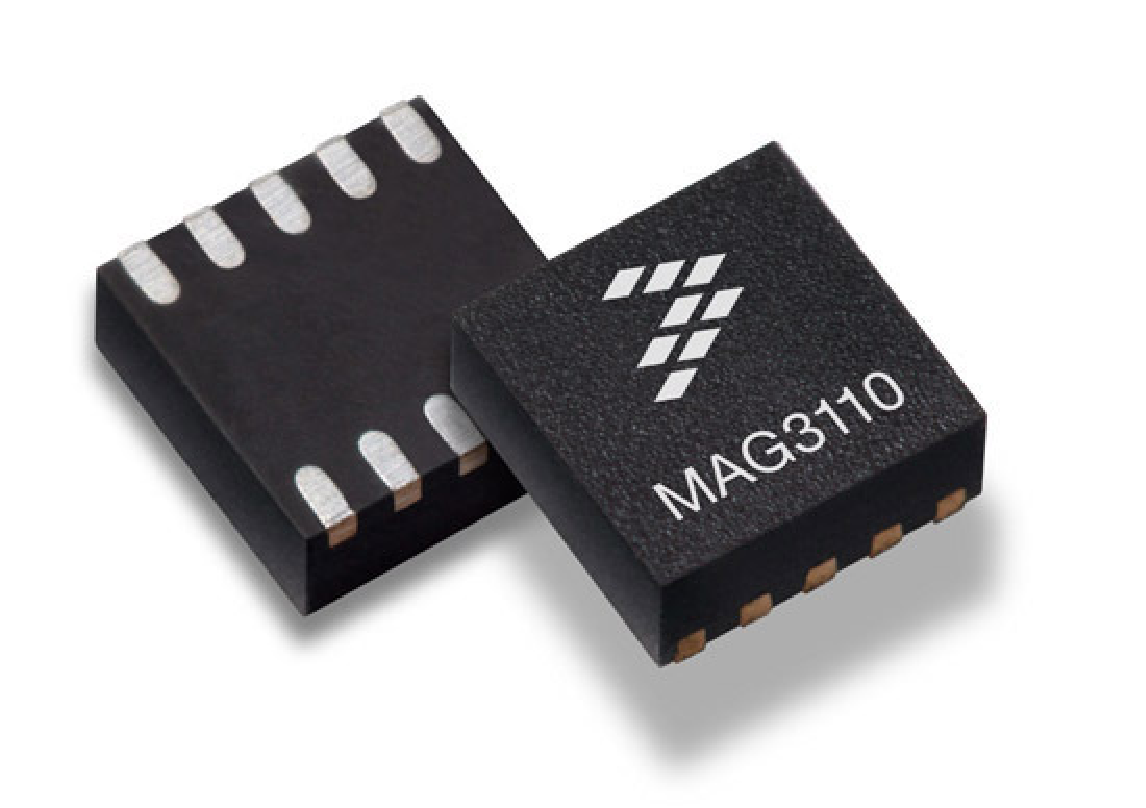
\includegraphics[height=45mm]{MGA}
        \end{center}
        \end{column}
    \end{columns}
\end{frame}


\begin{frame}
    \begin{center}
       {\zihao{2} Function}
    \end{center}


\end{frame}

\begin{frame}
    \frametitle{Function}
    \begin{columns}[onlytextwidth]
        \begin{column}{0.5\textwidth}
       
        Produce orientation independent accurate compass heading information

        \end{column}
    \begin{column}{0.5\textwidth}
            %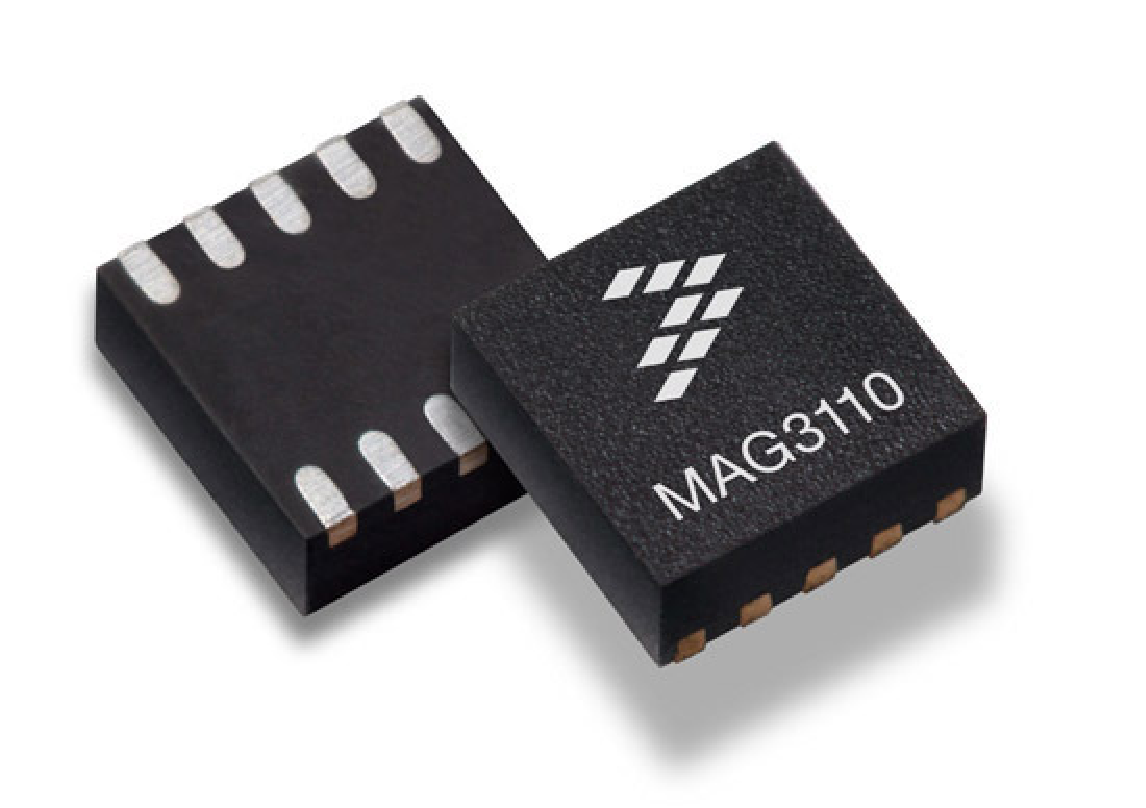
\includegraphics[height=45mm,width=\columnwidth]{MGA}\\
        \begin{center}
            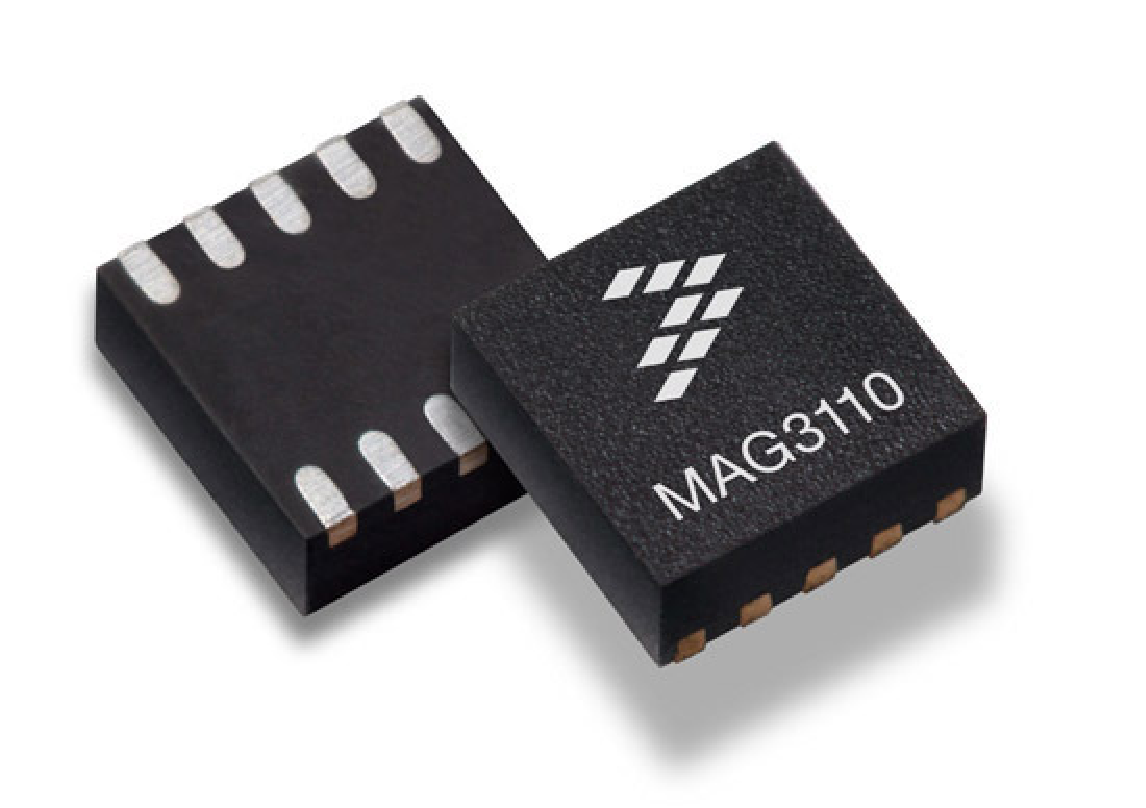
\includegraphics[height=45mm]{MGA}
        \end{center}
        \end{column}
    \end{columns}
\end{frame}


\begin{frame}
    \begin{center}
       {\zihao{2} Feature}
    \end{center}

\end{frame}

\begin{frame}
\frametitle{Feature}
    \begin{itemize}
        \pause
       \item Small ,Low-power, Digital 3-axis magnetometer
       \pause
       \item Output Data Rates (ODR) up to 80 Hz
       \pause
       \item Full Scale Range $\pm 1000\mu t$
       \pause
       \item Sensitivity of $0.10\mu t$
       \pause
       \item Noise down to $0.25\mu t $\quad rms
       \pause
       \item $I^{2}C$ digital output interface (operates up to 400 kHz Fast Mode)

    \end{itemize}

\end{frame}

\begin{frame}
    \begin{center}
       {\zihao{2} More Detail\ldots}
    \end{center}

\end{frame}

\begin{frame}
\frametitle{Block Diagram}
\begin{center}
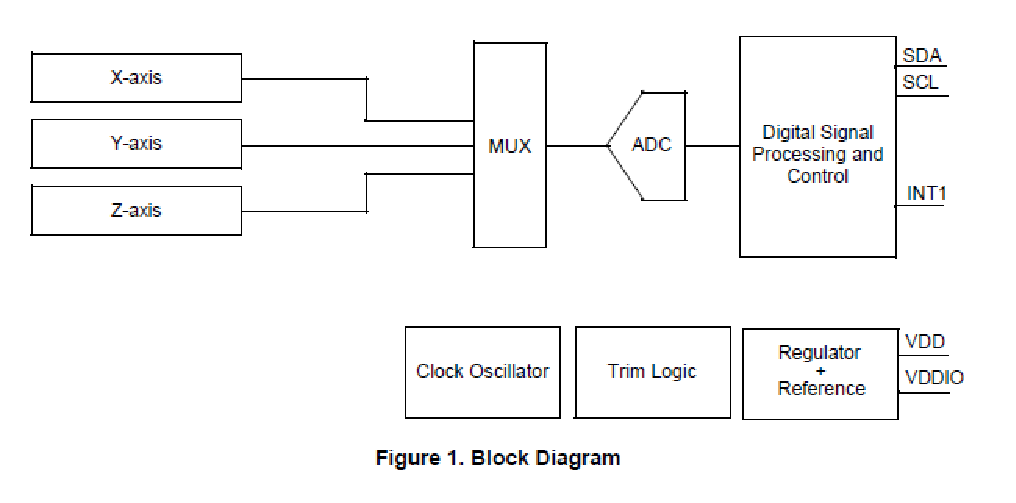
\includegraphics[height=45mm]{block}
\end{center}

\end{frame}

\begin{frame}
\frametitle{Pin Connections}
\begin{center}
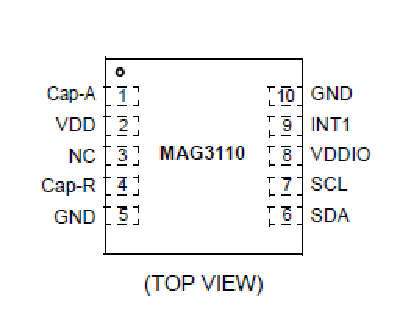
\includegraphics[height=40mm]{pin}
\end{center}
\end{frame}

\begin{frame}
\frametitle{Measurement Coordinate System}
\begin{center}
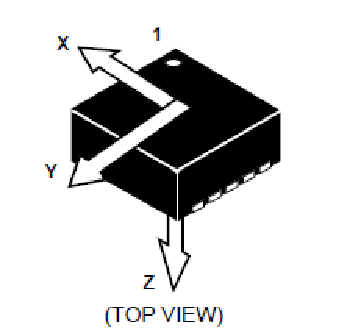
\includegraphics[height=40mm]{pin2}
\end{center}
\end{frame}

\begin{frame}
\frametitle{Electrical Connection}
\begin{center}
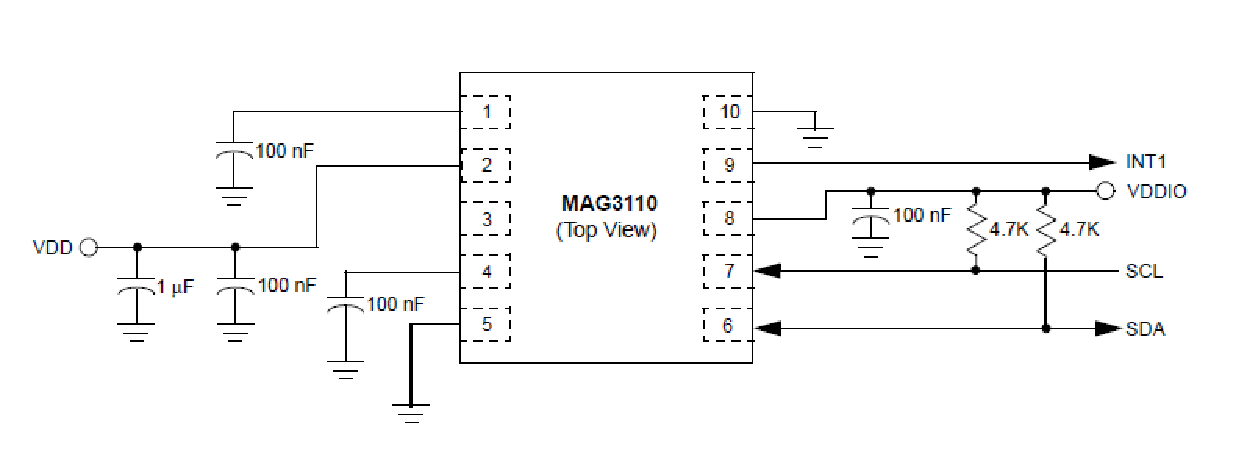
\includegraphics[height=40mm]{connection}
\end{center}
\end{frame}

\begin{frame}
    \begin{center}
       {\zihao{2} Application}
    \end{center}

\end{frame}

\begin{frame}
\frametitle{Application}

           \begin{itemize}
           \pause
                \item  Electronic Compass
                \pause
                 \item Dead-reckoning assistance for GPS backup
                 \pause
                \item Location-based Services
                \pause
                \item \ldots  \ldots
            \end{itemize}


\end{frame}


\section{Video}
\begin{frame}
\frametitle{Demo}
\movie[autostart,width=9cm,height=7cm,poster]{}{show.mp4}
%\movie[poster,width=5cm,height=4cm]{}{mag.mp4}
\end{frame}

\section{end}
\begin{frame}
\frametitle{The End}
\zihao{2}
\begin{center}
\textit{Thanks��}\\
SN : 1011061515
\end{center}
\end{frame}

\end{document} 